\documentclass[conference]{IEEEtran}
\usepackage[T1]{fontenc}
\usepackage{amsmath,amssymb,graphicx,booktabs,array,tabularx,xspace,cite,url}
\usepackage{balance}
\usepackage[hidelinks]{hyperref}
\newcolumntype{Y}{>{\raggedright\arraybackslash}X}
\newcommand{\Ehat}{\widehat E}
\newcommand{\AG}{\textsc{Agreement}}
% Generated by scripts/extract_results.py; do not hand-edit.
\newcommand{\BaselineRuns}{400\xspace}
\newcommand{\SuccessRuns}{366\xspace}
\newcommand{\BudgetRuns}{34\xspace}
\newcommand{\PrimaryModelPercent}{92.80\xspace}
\newcommand{\PrimaryEmpiricalPercent}{91.50\xspace}
\newcommand{\PrimaryCILower}{88.36\xspace}
\newcommand{\PrimaryCIUpper}{93.85\xspace}
\newcommand{\PrimaryDeviationPP}{1.30\xspace}
\newcommand{\TotalUpdates}{13,518\xspace}
\newcommand{\TotalEvaluations}{40,554\xspace}
\newcommand{\TotalMeasurements}{121,662\xspace}
\newcommand{\TotalShots}{124,581,888\xspace}
\newcommand{\ModelStates}{262,144\xspace}
\newcommand{\ModelTransitions}{755,176\xspace}
\newcommand{\GridPoints}{65,536\xspace}
\newcommand{\SuccessPoints}{8\xspace}
\newcommand{\GroundEnergy}{-0.702930394\xspace}
\newcommand{\ShotsPerGroup}{1,024\xspace}
\newcommand{\ShotsPerUpdate}{9,216\xspace}
\newcommand{\MaxShotsRun}{460,800\xspace}
\newcommand{\UpdateBound}{50\xspace}
\newcommand{\GridSize}{16\xspace}
\newcommand{\GapThreshold}{0.02\xspace}
\newcommand{\QuadraturePoints}{24\xspace}
\newcommand{\BootstrapSamples}{5,000\xspace}
\newcommand{\LogicalProperties}{7\xspace}
\newcommand{\DafnyChecks}{24\xspace}
\newcommand{\PModelMean}{33.111\xspace}
\newcommand{\PEmpiricalMean}{32.290\xspace}
\newcommand{\PMeanLow}{31.579\xspace}
\newcommand{\PMeanHigh}{32.995\xspace}
\newcommand{\PMeanRawP}{0.024\xspace}
\newcommand{\PMeanAdjustedP}{0.094\xspace}
\newcommand{\UnconditionalModel}{34.327\xspace}
\newcommand{\UnconditionalEmpirical}{33.795\xspace}
\newcommand{\EnergyError}{5.542\times 10^{-17}\xspace}
\newcommand{\StormDifference}{1.110\times 10^{-16}\xspace}
\newcommand{\QuadratureCorrection}{5.090\times 10^{-8}\xspace}
\newcommand{\DetectablePP}{3.62\xspace}
\newcommand{\LegacyLogicalProperties}{41\xspace}
\newcommand{\PhaseQueries}{18\xspace}
\newcommand{\TimingMeasured}{300\xspace}
\newcommand{\TimingWarmup}{50\xspace}
\newcommand{\TimingWarmupsPerCell}{5\xspace}
\newcommand{\TimingRepetitions}{30\xspace}
\newcommand{\TimingBaselineFinal}{0.215\xspace}
\newcommand{\TimingVerifiedFinal}{1.876\xspace}
\newcommand{\TimingAddedFinal}{1.661\xspace}
\newcommand{\TimingRelativeFinal}{771.84\xspace}
\newcommand{\NoisyRuns}{400\xspace}
\newcommand{\NoisySuccess}{347\xspace}
\newcommand{\NoisyPercent}{86.75\xspace}
\newcommand{\ScaleMaxStates}{1,741,676\xspace}
\newcommand{\ScaleMaxTransitions}{4,889,851\xspace}
\newcommand{\FaultRuns}{50\xspace}
\newcommand{\FaultClasses}{5\xspace}
\newcommand{\FaultRepetitions}{10\xspace}
\newcommand{\LogicalScalingPairs}{$(3,2)$, $(5,3)$, $(10,5)$, $(20,10)$\xspace}
\newcommand{\LogicalScalingTimes}{0.04, 0.02, 0.03, 0.07\xspace}
\newcommand{\EstimatorQubits}{2\xspace}
\newcommand{\EstimatorTerms}{4\xspace}
\newcommand{\EstimatorRecords}{25\xspace}
\newcommand{\HeisenbergQubits}{14\xspace}
\newcommand{\HeisenbergTerms}{287\xspace}
\newcommand{\HeisenbergRecords}{60\xspace}

\author{}
\title{Formal Verification in Hybrid Quantum--Classical Computing Systems:\\A Two-Stage Contract Framework for VQE}
\begin{document}
\maketitle
\begin{abstract}
The variational quantum eigensolver (VQE) couples classical decisions to uncertain quantum measurement estimates. We organize its verification around a shared execution model and a system-level contract library. Logical, numeric, and probabilistic contracts retain their own formalisms: NuXmv checks a bounded controller, Dafny proves real and integer kernels under assumptions, and Storm checks a Gaussian discrete-time Markov chain. A frozen pre-execution assurance record links these results to runtime evidence from the same canonical instance. In the final matched experiment, \BaselineRuns finite-shot executions satisfy the observed logical and numeric obligations, with the prospective scope of termination and measurement accounting stated separately. The Gaussian model predicts \PrimaryModelPercent\% success by \UpdateBound updates; \SuccessRuns executions succeed, giving \PrimaryEmpiricalPercent\% with a 95\% Wilson interval of [\PrimaryCILower\%, \PrimaryCIUpper\%]. Conditional update and shot costs are statistically compatible after adjustment for the supporting comparisons; an earlier marginal-interval disagreement was a statistical false alarm. Controlled faults distinguish observed violations, changed assumptions, and incomplete evidence. Retained layer-specific studies quantify model growth and runtime cost under their own configurations. The results support contract-wise cross-stage consistency on a two-qubit benchmark, while keeping model checking, mathematical proof, observed conformance, and statistical evidence within their respective scopes.
\end{abstract}
\begin{IEEEkeywords}
VQE, formal verification, runtime verification, probabilistic model checking, contract traceability.
\end{IEEEkeywords}

\section{Introduction}
\label{sec:introduction}
VQE estimates a Hamiltonian expectation using a parameterized quantum state and adjusts the parameters with a classical optimizer~\cite{peruzzo2014,mcclean2016}. Correct interaction requires more than a plausible final energy. Measurements must belong to the current candidate; aggregation must include the declared observables and coefficients; the optimizer must consume the values actually validated; and stopping must respect the declared policy. Finite-shot uncertainty introduces a different question: how often does the search reach its target within the resource bound?

These obligations call for different verification objects. A controller model captures ordering but abstracts arithmetic and measurement outcomes. A numeric proof establishes a calculation under input assumptions. A probabilistic model describes uncertain selections. Runtime evidence determines whether corresponding obligations hold in instrumented executions. Treating their results as interchangeable would obscure both the guarantees and the remaining assumptions.

The methodological principle is:
\begin{quote}
The contract library defines what the VQE implementation is expected to satisfy. Pre-execution verification establishes these contracts prospectively, while runtime verification determines whether the corresponding obligations hold for concrete executions.
\end{quote}
The principle does not imply that every obligation is fully proved at each stage. Contract matching must record the actual prospective subclaim, its assumptions, and the strength of the runtime counterpart.

We make three contributions. First, we define a two-stage architecture with a canonical instance, a family-owned contract library, and a frozen assurance record. Second, we explain how logical, numeric, and probabilistic obligations connect to runtime evidence without forcing a common formalism. Third, we evaluate those connections contract-wise using the final audited execution archive, controlled faults, and retained layer-specific cost studies. The paper asks: (RQ1) how are obligations organized around the shared execution model; (RQ2) what does each implemented layer establish; (RQ3) do the matched prospective and runtime results agree within their scopes; and (RQ4) what costs and fault behaviors are observed? RQ3 concerns consistency of evidence, rather than a proved theorem composing all tools.

Section~\ref{sec:model} introduces the execution model and contract library. Section~\ref{sec:methods} gives each layer's technical meaning and procedure. Section~\ref{sec:individual} evaluates the layers under their corresponding setups. Section~\ref{sec:crosslayer} then evaluates their relationships collectively using the matched experiment.

\section{Shared Execution Model and Contract Library}
\label{sec:model}
\subsection{Execution and Contract Semantics}
The shared execution view is a labeled transition system whose modes are initialization, preparation, measurement, aggregation, validation, optimizer commitment, stopping checks, and terminal closure. Its state retains a run identifier, candidate and evaluation identities, parameters, available measurement groups, validation readiness, update count, and resource accounting. Concrete identifiers strengthen the abstract controller's counters and epoch flags; their correspondence is an implementation mapping, not a machine-checked refinement theorem.

For a Pauli decomposition $H=\sum_i c_iP_i$, VQE evaluates
\begin{equation}
 E(\theta)=\langle\psi(\theta)|H|\psi(\theta)\rangle,
 \qquad \Ehat(\theta)=\sum_i c_i\hat e_i.
 \label{eq:energy}
\end{equation}
Each contract records a family, obligation, pre-execution check, runtime counterpart, assumptions, and comparison rule. The implemented library is \texttt{config/contracts.json}. It documents these links; it is not a generator translating one specification into all three formalisms. Logical and numeric contracts apply at run level. Probabilistic contracts apply to repeated executions of a declared process.

Figure~\ref{fig:architecture} shows the two stages. Pre-execution verification produces models, proof logs, and quantitative predictions before the designated execution begins. The assurance record freezes configuration, source hashes, tool identities, and artifact hashes. Stage 2 refuses execution when this evidence no longer matches. Runtime observations then support contract matching and verdict agreement. Changing a model or implementation requires a new assurance record and output directory; this feedback is manual.

\begin{figure*}[!t]
\centering
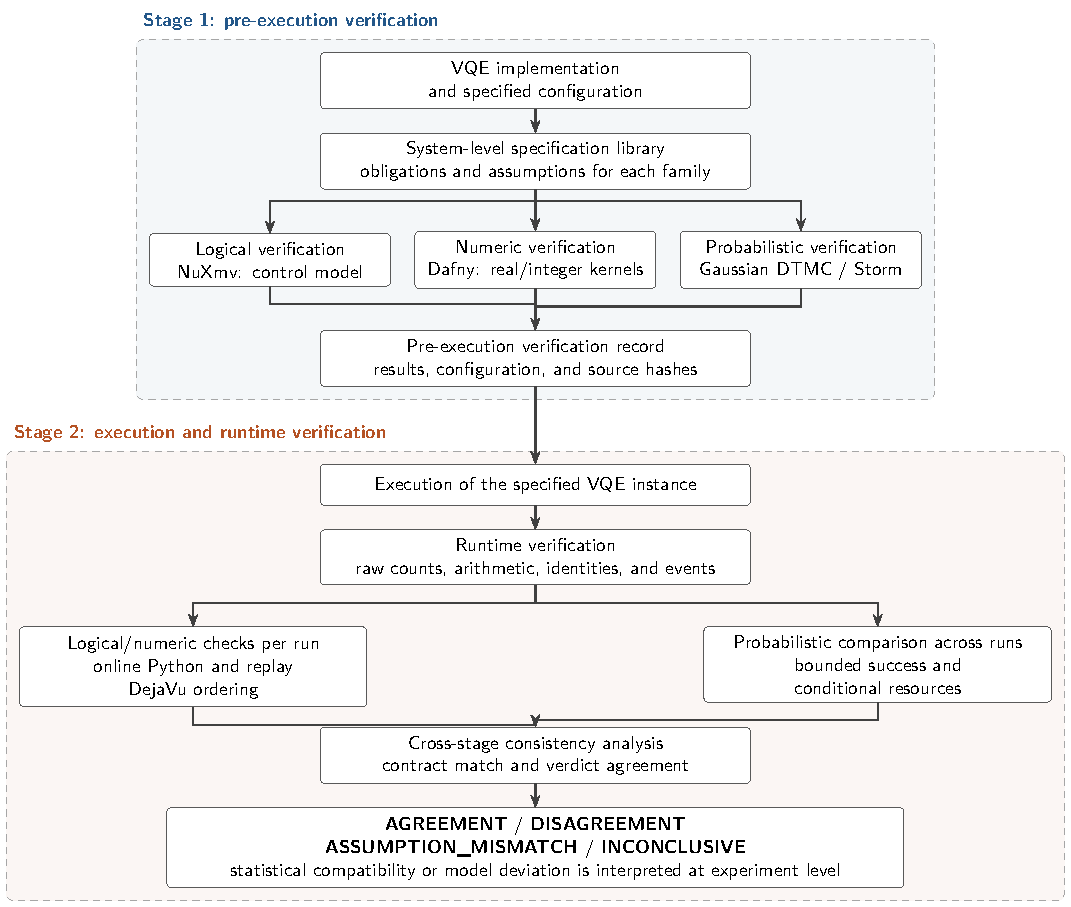
\includegraphics[width=.94\textwidth]{figures/architecture.pdf}
\caption{Two-stage verification architecture for the canonical VQE instance. The contract families retain heterogeneous verification objects. The frozen record precedes execution; runtime checking combines run-level logical/numeric evidence with probabilistic evidence across repeated executions. The displayed verdict names match the implementation. A probabilistic disagreement denotes a model discrepancy only when assumptions and the statistical decision rule justify that interpretation. The architecture supplies traceability rather than an equivalence among NuXmv, Dafny, and Storm.}
\label{fig:architecture}
\end{figure*}

Table~\ref{tab:mapping} gives the contract mapping. A numeric-to-runtime match is established by interpreting concrete counts and optimizer inputs as the mathematical inputs of the kernel contract, checking its preconditions, and comparing the observed output to the declared arithmetic. It does not require the Python implementation to be verified by Dafny. For probabilistic matching, the runtime counterpart is an estimate over repeated executions, rather than an assertion that every run succeeds.

\begin{table*}[!t]
\centering\footnotesize
\caption{System-level contract traceability. Each row connects a prospective object to concrete evidence and its interpretation. Assumptions and prospective gaps are part of the mapping.}
\label{tab:mapping}
\begin{tabularx}{\textwidth}{@{}p{.04\textwidth}>{\raggedright\arraybackslash}p{.20\textwidth}>{\raggedright\arraybackslash}p{.25\textwidth}>{\raggedright\arraybackslash}p{.25\textwidth}Y@{}}
\toprule
ID & Obligation & Pre-execution verification & Runtime evidence & Cross-stage interpretation \\
\midrule
L1 & Complete measurements before energy aggregation & NuXmv: aggregation implies three group completions & Unique candidate/group records; DejaVu past-group facts & Ordering agreement when required evidence is present \\
L2 & Candidate validation before optimizer commitment & NuXmv: selection/commit requires three ready candidates & Three validation events precede commit; consumed scores & Agreement of ordering; online enforcement is fail-stop \\
L3 & Current evaluation and parameter provenance & NuXmv: epoch equality and readiness reset & Run/update/evaluation identities, indices, angles, successors & Runtime checks strengthen the epoch abstraction \\
L4 & Terminal closure and declared stopping reason & NuXmv: absorbing terminals and budget bounds only & No later activity; reason checked against oracle/budget & Qualified agreement for shared subclaims; reason is runtime-only \\
N1 & Expectations consistent with raw counts & Dafny normalization kernel and range bound & Exact parity reconstruction and count totals & Agreement under trusted basis and parity mapping \\
N2 & Energy uses declared coefficients and measurements & Dafny contribution, weighted-sum, and interval kernels & Rational reference versus contributions, total energy, actual optimizer input & Arithmetic agreement within frozen tolerance \\
N3 & Physical shots counted consistently & Dafny natural-number list accumulation & Unique group executions, allocations, cumulative totals & Agreement under group-identity assumptions; changed shots invalidate the stochastic setup \\
N4 & Valid candidates and deterministic selection & Dafny modular wrap and integer argmin/tie priority & Recomputed candidate indices, scores, chosen successor & Agreement under trusted angle/gate interpretation \\
P1 & Bounded success probability & Storm reachability of the Gaussian DTMC & First-success frequencies and Wilson intervals & Statistical compatibility under matched conditions \\
P2 & Updates conditional on bounded success & Python propagation of the same Gaussian kernel & Mean first-success update and bootstrap interval & Supporting, multiplicity-adjusted comparison \\
P3 & Shots conditional on bounded success & Fixed shot allocation times P2 & Successful-path shots; fixed shots/update & Derived from P2, not independent evidence \\
\bottomrule
\end{tabularx}
\end{table*}

\subsection{Canonical Instance and Frozen Boundary}
\label{sec:canonical}
The matched instance uses the following two-qubit benchmark operator, written in $q_1\otimes q_0$ order:
\begin{equation}
 H=0.398\,YZ-0.398\,ZI-0.0113\,ZZ+0.181\,XX.
 \label{eq:hamiltonian}
\end{equation}
The repository retains legacy ``h2'' names, but the operator has no documented molecular mapping and is not presented as a molecular-hydrogen Hamiltonian. Its reference minimum eigenvalue is $E_{\rm ref}=\GroundEnergy$ in the operator's numerical units. We use the same operator across the matched projections, without assigning chemical-accuracy meaning to the target.

The circuit applies H to both qubits, the first pair of RZ rotations, Y to both, CX$(0\!\to\!1)$, H to both, the second pair of RZ rotations, and Y to both. Four integer indices $z$ give angles $\theta_j=2\pi z_j/\GridSize$, with wrap-around. The optimizer cycles through coordinates; each update remeasures the current, minus-one, and plus-one candidates and chooses the smallest integer energy score. Ties prefer current, then minus, then plus. The integer coefficients are the declared decimal coefficients scaled by $10^4$.

\begin{table}[!t]
\centering\footnotesize
\caption{Final matched configuration from the sealed assurance record. An update contains three candidate evaluations and nine group executions.}
\label{tab:configuration}
\begin{tabularx}{\columnwidth}{@{}p{.43\columnwidth}Y@{}}
\toprule
Item & Declared value \\
\midrule
Parameter grid & $z\in\{0,\ldots,\GridSize-1\}^4$; \GridPoints points \\
Initial index & $(3,11,6,14)$ \\
Coordinate cycle & $(0,1,2,3)$ \\
Measurement groups & $\{ZI,ZZ\}$, $\{YZ\}$, $\{XX\}$ \\
Shots/group/candidate & \ShotsPerGroup \\
Physical shots/update & \ShotsPerUpdate \\
Update bound & $K=\UpdateBound$ \\
Maximum shots/run & \MaxShotsRun \\
Success & $E_{\rm ideal}(z)-E_{\rm ref}\leq\GapThreshold$ \\
Baseline executions & \BaselineRuns; separate seeded streams \\
Environment & Ideal Born probabilities; finite-shot multinomial counts \\
Numeric tolerance & $10^{-12}$ for energy and expectations \\
Gaussian integration & \QuadraturePoints-node Gauss--Hermite quadrature \\
Intervals & 95\% Wilson; \BootstrapSamples bootstrap resamples \\
\bottomrule
\end{tabularx}
\end{table}

Table~\ref{tab:configuration} fixes the boundary. The run stops on first ideal-energy success or normal budget exhaustion; an online contract problem gives an error closure. The success oracle uses exact simulation of the selected point. It is a benchmarking predicate available to this simulator, not a hardware-observed stopping certificate or an energy-stability policy. There are \SuccessPoints successful grid points. Each failed run remains in the probability denominator and consumes its budget.

\section{Technical Meaning and Procedure of Each Layer}
\label{sec:methods}
\subsection{Logical Verification}
NuXmv~\cite{nuxmv} checks a finite controller with measurement-group counters, candidate readiness, an update counter, and epoch flags. Measurement and environment outcomes are nondeterministic; numeric energies and quantum states are abstracted. Representative LTL obligations are
\begin{align}
 &\mathbf G(\mathrm{aggregate}\Rightarrow\mathrm{groups}=3),\nonumber\\
 &\mathbf G(\mathrm{select}\lor\mathrm{commit}\Rightarrow\mathrm{ready}=3),\nonumber\\
 &\mathbf G(\mathrm{commit}\Rightarrow\mathrm{energyEpoch}=\mathrm{epoch}).
 \label{eq:logical}
\end{align}
Readiness resets at the next update; terminal states are absorbing. The procedure generates the controller from the frozen bound, runs NuXmv, and stores every returned property and verdict. The result is exhaustive for the encoded model.

L4 requires special care. The final property set checks terminal absorption, that a budget-terminal state has the bound counter, and that commits occur below the bound. It does not establish that success and budget exhaustion must take their intended terminal branches. The audit found that changing either branch to abort leaves these properties true. Consequently, the paper reports only the verified subclaim prospectively. Runtime reason checks are additional evidence. The controller's presence of separate terminal branches does not itself supply the missing property.

\subsection{Numeric Verification and Its Runtime Match}
\label{sec:numeric}
Dafny~\cite{dafny} proves kernels with mathematical real and integer semantics. A normalization routine assumes a positive shot count and an admissible event count. Weighted-sum routines assume matching term sequences and expectations in $[-1,1]$, and establish
\begin{equation}
 -\sum_i|c_i|\leq\sum_i c_i\hat e_i\leq\sum_i|c_i|.
 \label{eq:numericbound}
\end{equation}
Additional kernels accumulate natural-number shot records, preserve the grid under modular wrap, and choose the minimum integer score with the declared tie priority. Verification logs are frozen with the source modules.

Runtime matching uses raw measurements rather than assuming a reported expectation is correct. For outcome counts $n_{g,o}$ in group $g$, let $s_{i,o}\in\{-1,+1\}$ be the declared Pauli parity. The reference values are
\begin{equation}
 \hat e_i^{\rm ref}=\frac{\sum_o s_{i,o}n_{g,o}}{\sum_o n_{g,o}},
 \qquad E^{\rm ref}=\sum_i c_i\hat e_i^{\rm ref}.
 \label{eq:runtime-reference}
\end{equation}
The checker reconstructs these as exact rational numbers and compares the concrete floating-point expectations, contributions, and energy to them within the frozen tolerance. It also checks the integer scores and the actual values recorded as consumed by the optimizer. Thus the link is a shared mathematical obligation instantiated on observed inputs and outputs. There is no proved compiler refinement from the Dafny kernels to Python floating-point operations.

The boundaries matter. The normalization lemma uses the single-event count form; multi-qubit parity interpretation is trusted. The shot-accumulation proof establishes a list sum; it does not prove that list entries are unique physical executions. Runtime identities and completeness checks discharge these observational conditions under faithful instrumentation. Missing inputs yield incomplete evidence; changed shot allocations invalidate the probabilistic configuration. Proving consequences of a valid-record predicate does not prove that an arbitrary record is valid.

\subsection{Probabilistic Verification}
\label{sec:probabilistic}
For each candidate, the Gaussian abstraction matches the ideal mean energy and the shot-estimator variance. Terms measured in the same group retain their covariance:
\begin{equation}
 \sigma^2(z)=\frac{1}{N_g}\sum_g
 \operatorname{Var}_{\rm Born}\!\left(\sum_{i\in g}c_i s_i\right),
 \label{eq:variance}
\end{equation}
where all groups receive $N_g=\ShotsPerGroup$ shots. Groups, candidate measurements, and repeated executions are independent; terms within a group need not be. Approximating a candidate energy by $X_j\sim\mathcal N(\mu_j,\sigma_j^2)$ gives its selection probability
\begin{equation}
 \Pr(j=\operatorname*{argmin}_\ell X_\ell)
 =\int f_j(x)\prod_{\ell\ne j}[1-F_\ell(x)]\,dx.
 \label{eq:selection}
\end{equation}
The implementation evaluates this integral by configured quadrature and a normal-CDF approximation, then normalizes rows. The continuous model gives ties probability zero; discrete finite-shot execution applies the explicit tie rule.

The DTMC state is the parameter-grid point and next coordinate phase. Success states are absorbing. Storm~\cite{storm} checks
\begin{equation}
 p_G(k)=\Pr_G(T\leq k)
 \quad\text{using }\mathrm{P}_{=?}[\mathrm F^{\leq k}\ \mathrm{success}].
 \label{eq:reachability}
\end{equation}
This is exhaustive model checking of the constructed Gaussian DTMC, not the physical finite-shot process. Python forward propagation of the same kernel produces the full cumulative curve and first-success distribution. P2 is $\mathbb E_G[T\mid T\leq K]$; P3 multiplies P2 by the fixed shots per update. These conditional quantities are not Storm reward-query outputs and exclude failed paths. Total expenditure is reported separately. No certified approximation-error bound follows from quadrature row normalization or agreement between two computations of the same model.

\subsection{Runtime Verification}
\label{sec:runtime}
The canonical executor emits preparation and update context, raw group counts, candidate evaluations, numeric-valid events, optimizer commits, and terminal closure. Python checks each emitted event synchronously and stops the run when a problem appears. It checks current identities, complete measurements, arithmetic, consumed scores, successor parameters, resource totals, and terminal reasons. The implementation records a commit and assigns the successor before checking acceptance; its protection is emit-then-check fail-stop, not a separate pre-authorization protocol.

Saved traces are replayed with the same Python checker class. Online/replay agreement supports deterministic reconstruction of those verdicts, not independent implementation correctness. A separately compiled DejaVu monitor~\cite{dejavu} batch-replays five temporal projections covering group ordering, validations before commit, energy after update start, validation after energy, and no activity after stop. It is an independent ordering check with narrower coverage, and does not verify arithmetic or authenticate the source of counts. The earlier runtime implementation used an ask/tell acknowledgment protocol; its separate evidence is evaluated below.

\section{Individual Layer Evaluation}
\label{sec:individual}
\subsection{Evidence Selection and Experimental Boundaries}
The collective experiment uses exclusively the final run designated in the artifact index and independently audited. Development and earlier primary directories reuse the full-run seeds and are not pooled as independent observations. The retained studies in this section answer layer-specific questions under their own configurations. Their different controllers, stopping rules, measurement strategies, and timing boundaries are not treated as one canonical execution.

The final archive was sealed before its designated runtime execution. Earlier development executions had already exposed the same seeded trajectories; this was an engineering iteration rather than a blinded confirmatory study. The paper's P2/P3 interpretation is a reporting correction after the audit, with primary data and frozen experimental sources preserved. The reproducibility bundle records source hashes and generates numerical text, tables, and plots programmatically.

\subsection{Logical and Numeric Outcomes}
The earlier refined controller has \LegacyLogicalProperties true properties in its saved NuXmv output and \PhaseQueries positive phase-reachability queries in the separate archive. Its budget-abort naming differs from the matched controller's normal budget closure. Table~\ref{tab:logical-scaling} reports its bounded configurations and single wall-clock measurements. These small timings are not evidence of a general scalability law or of cost as quantum-state dimension grows.

\begin{table}[!t]
\centering\footnotesize
\caption{Retained refined-controller evaluation. Each row has one local timing measurement; this model is distinct from the final matched controller.}
\label{tab:logical-scaling}
\begin{tabular}{@{}rrrrr@{}}\toprule
Updates & Terms & True & False & Time (s) \\
\midrule
3 & 2 & 41 & 0 & 0.04 \\
5 & 3 & 41 & 0 & 0.02 \\
10 & 5 & 41 & 0 & 0.03 \\
20 & 10 & 41 & 0 & 0.07 \\
\bottomrule


\end{tabular}
\end{table}

For the canonical matched instance, \LogicalProperties logical properties hold and the three Dafny verification invocations report \DafnyChecks verified units with zero errors. These are tool-reported verification units, not a count of independent system-level properties. Their distribution across modules and their correspondence to N1--N4 are retained in the evidence manifest.

The earlier numeric checker also supports an executed Estimator trace and a larger exact-estimate trace, replayed with the later recorded checker in Table~\ref{tab:numeric-traces}. The Estimator trace lacks raw measurement counts, so it cannot establish the raw-count reconstruction now available in the matched experiment. The Heisenberg trace illustrates acceptance of a larger term list; it provides no timing-scaling or optimizer-success theorem. Synthetic fixtures are not described as executed molecular instances.

\begin{table}[!t]
\centering\footnotesize
\caption{Retained numeric traces replayed with checker version 2.0. PASS denotes record conformance under that checker; raw counts are unavailable in the Estimator trace.}
\label{tab:numeric-traces}
\begin{tabular}{@{}lrrrr@{}}\toprule
Trace & Qubits & Terms & Records & Verdict \\
\midrule
Two-qubit Estimator & 2 & 4 & 25 & PASS \\
Heisenberg & 14 & 287 & 60 & PASS \\
\bottomrule


\end{tabular}
\end{table}

\subsection{Probabilistic Model Size and Cost}
\label{sec:modelcost}
The retained scalability study builds a reachable, time-unrolled DTMC for each bound. It merges successful paths into an absorbing success state and horizon-exhausted paths into an absorbing timeout state. Figure~\ref{fig:storm-scalability} shows its recorded states and transitions. At the largest bound, it contains \ScaleMaxStates states and \ScaleMaxTransitions transitions. This is a different representation from the final homogeneous grid/coordinate-phase DTMC, whose size is fixed at \ModelStates states and \ModelTransitions transitions. Increasing a reachability-query horizon on the latter does not create the time-unrolled growth shown in the figure.

\begin{figure}[!t]
\centering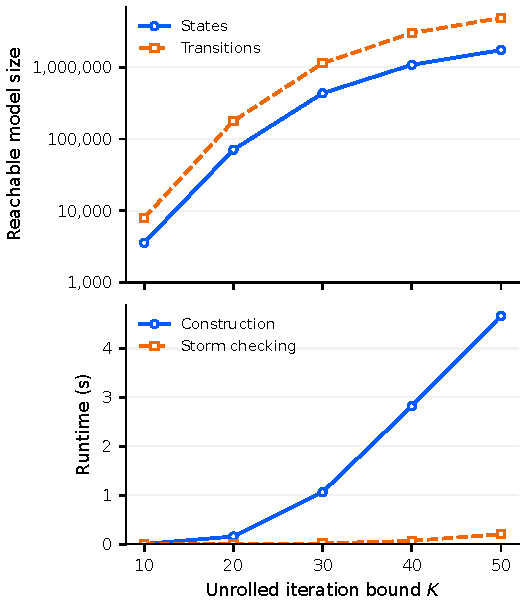
\includegraphics[width=\columnwidth]{figures/storm-scalability.pdf}
\caption{Reachable states and transitions in the retained time-unrolled Gaussian DTMC study, at the declared grid and shot allocation. The vertical axis is logarithmic; each marker is an archived model size. This representation expands the reachable update-depth history and differs from the fixed-size homogeneous phase DTMC used in the final matched experiment.}
\label{fig:storm-scalability}
\end{figure}

Table~\ref{tab:storm-cost} separates construction and checking. Construction excludes Gaussian-kernel preparation; checking is the median of the recorded tool-reported repetitions and excludes parsing. A displayed zero is below reporting resolution. The archive retains per-depth state counts, timings, the CSV, metadata, and generation source, but not the exported explicit scalability models. Accordingly, this supports the recorded model-growth and cost measurements, with a weaker raw-model audit trail than the final retained DTMC.

\begin{table}[!t]
\centering\footnotesize
\caption{Retained time-unrolled model cost. Construction is one measurement; checking is the median of three tool-reported timings.}
\label{tab:storm-cost}
\begin{tabular}{@{}rrr@{}}\toprule
$K$ & Construction (s) & Checking (s) \\
\midrule
10 & 0.008 & 0.000 \\
20 & 0.161 & 0.002 \\
30 & 1.067 & 0.020 \\
40 & 2.821 & 0.072 \\
50 & 4.663 & 0.206 \\
\bottomrule


\end{tabular}
\end{table}

\subsection{Runtime Cost and Hardware Evidence}
The completed September runtime cost study has \TimingWarmup warm-ups and \TimingMeasured measured runs. Each condition and evaluation count has \TimingWarmupsPerCell warm-ups followed by \TimingRepetitions measured repetitions. It uses a StatevectorSampler, separate measurement submissions per Pauli term, an ask/tell pattern-search optimizer, and the recorded stability policy. Reusing the workload seed holds the sampled trajectory fixed while repetitions measure timing variation. This is separate from the final cyclic-grid experiment.

Figure~\ref{fig:runtime-overhead} and Table~\ref{tab:runtime-cost} report total runtime and the difference of condition medians. The verified timing includes setup, monitor startup, online checking/acknowledgments, and finalization; archived fidelity computation, artifact writing outside the declared boundary, and offline replay are excluded. Bootstrap samples independently resample each condition's measured times. The resulting intervals describe uncertainty in timing summaries for this workload, not variation across independent optimization trajectories.

\begin{figure}[!t]
\centering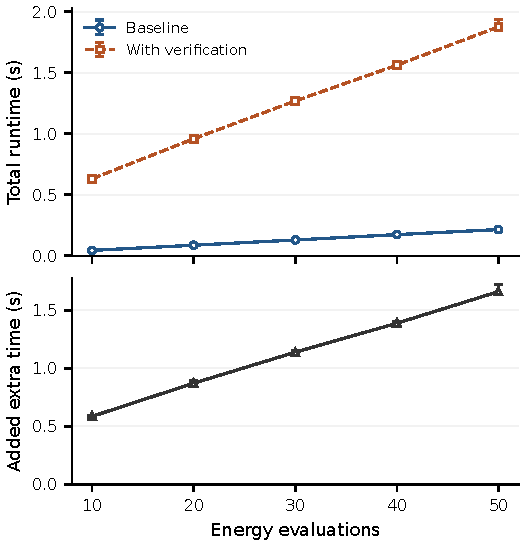
\includegraphics[width=\columnwidth]{figures/runtime-overhead.pdf}
\caption{Retained simulator runtime cost under the separate ask/tell runtime implementation. Top: baseline and verified medians. Bottom: verified median minus baseline median. Error bars are 95\% percentile bootstrap intervals from 10,000 independent-condition resamples, using \TimingRepetitions measured runs per condition/count after \TimingWarmupsPerCell warm-ups. Timing includes setup, online monitoring, and finalization; fidelity analysis and offline replay are excluded. Repetitions use the same workload seed.}
\label{fig:runtime-overhead}
\end{figure}

\begin{table}[!t]
\centering\footnotesize
\caption{Timing medians and added cost in seconds. The interval applies to the difference of independent condition medians.}
\label{tab:runtime-cost}
\begin{tabular}{@{}rrrrl@{}}\toprule
Evals. & Baseline & Verified & Added & Added 95\% CI \\
\midrule
10 & 0.044 & 0.630 & 0.586 & [0.579, 0.592] \\
20 & 0.087 & 0.959 & 0.872 & [0.863, 0.891] \\
30 & 0.130 & 1.268 & 1.139 & [1.119, 1.156] \\
40 & 0.174 & 1.562 & 1.388 & [1.366, 1.406] \\
50 & 0.215 & 1.876 & 1.661 & [1.633, 1.721] \\
\bottomrule


\end{tabular}
\end{table}

At the largest tested count, the baseline median is \TimingBaselineFinal s, the verified median is \TimingVerifiedFinal s, and the added median time is \TimingAddedFinal s (\TimingRelativeFinal\% relative increase). These measurements show substantial relative overhead on a fast simulator; they do not establish the final canonical experiment's overhead or larger-workload scaling. The final matched archive has no repeated uninstrumented timing condition, and numeric verification has no systematic cost study.

The retained runtime archive also contains separately configured sampled simulator and \texttt{ibm\_marrakesh} executions. Table~\ref{tab:hardware} reports their verified measurements and online/replay outcomes. Both close at the evaluation budget rather than certify ideal-energy success. Their acceptance supports observed event, arithmetic, resource, and evidence conformance. A hardware result with backend noise and a different optimizer is not a matched validation of the Gaussian search model.

\begin{table}[!t]
\centering\footnotesize
\caption{Separate runtime simulator and hardware evidence, verified against archived hashes and reports. ``pass/pass'' denotes online/replay conformance; both use budget termination.}
\label{tab:hardware}
\begin{tabular}{@{}lrrrl@{}}\toprule
Execution & Evals. & PUBs & Shots & Online/replay \\
\midrule
statevector\_sampler & 50 & 200 & 204,800 & pass/pass \\
ibm\_marrakesh & 50 & 200 & 204,800 & pass/pass \\
\bottomrule


\end{tabular}
\end{table}

\section{Cross-Layer Relationships and Agreement}
\label{sec:crosslayer}
\subsection{Experiment Goals and Comparison Procedure}
The collective experiment asks whether the frozen prospective subclaims remain consistent with concrete evidence when circuit, operator, parameters, candidate rule, measurement groups, shot allocation, success predicate, and bound are matched. It also tests how controlled faults affect the contract vector. It does not test chemical validity, prove physical measurements, establish general optimizer convergence, or combine the tools into one formal semantics.

Stage 1 generates and checks the controller, verifies the numeric modules, constructs the Gaussian kernel and DTMC, runs Storm at declared checkpoints, compiles the temporal monitor, and seals the assurance record. Stage 2 executes the identical recorded configuration, stores raw counts and all consumed optimizer values, and performs online and replay checking. The comparison validates the seal and trace hashes and reports each contract separately. A numerical tolerance is part of deterministic conformance; confidence intervals express statistical uncertainty and have a different role.

The implementation labels observed satisfaction \texttt{AGREEMENT}, violations \texttt{DISAGREEMENT}, invalid assumptions \texttt{ASSUMPTION\_MISMATCH}, and missing or unavailable checks \texttt{INCONCLUSIVE}. We interpret a disagreement according to the contract and evidence. A probabilistic deviation can concern the Gaussian model only after its matched-assumption boundary is established. An individual failed stochastic search is not a violation of P1. The software gates execution on successful Stage 1 results, so it does not evaluate the complete matrix of failed prospective checks against runtime outcomes.

For P1, the final bound is the designated primary comparison. We report pointwise Wilson intervals for all declared checkpoints. For the informative supporting comparisons, the audit-recommended analysis computes two-sided score-test $p$-values for the nonzero checkpoint probabilities and a normal-approximation test for the successful-run update mean, then applies Holm adjustment to this family. The zero-probability early checkpoints are structurally uninformative; P3 duplicates P2 and is not an additional test. This post-audit adjustment corrects interpretation without replacing the observations or claiming a preregistered equivalence margin.

\subsection{Logical and Numeric Contract Agreement}
Table~\ref{tab:contract-results} gives the prospective subclaim and runtime count for every logical and numeric contract. All observed baseline obligations agree on \BaselineRuns runs, subject to the mapping qualifications. This is observed conformance, not proof of all Python executions. In particular, L4 agreement covers the shared terminal-absorption and bound conditions; the stronger termination-reason check has runtime evidence alone.

\begin{table*}[!t]
\centering\footnotesize
\caption{Final contract-wise logical/numeric results. The listed prospective subclaims have successful tool outputs; the runtime column counts agreeing baseline runs. Agreement is interpreted under Table~\ref{tab:mapping}'s assumptions. L4 does not carry a prospective proof of termination reasons.}
\label{tab:contract-results}
\begin{tabularx}{\textwidth}{@{}p{.045\textwidth}p{.44\textwidth}p{.14\textwidth}Y@{}}\toprule
ID & Prospectively established scope & Runtime agreement & Cross-stage classification \\
\midrule
L1 & Group-completeness counter & 400/400 & Agreement under mapping \\
L2 & Validation-readiness counter & 400/400 & Agreement under mapping \\
L3 & Epoch and readiness reset & 400/400 & Agreement under mapping \\
L4 & Terminal absorption and budget bounds & 400/400 & Qualified agreement \\
N1 & Normalization kernel with parity assumed & 400/400 & Agreement under mapping \\
N2 & Real weighted sum and bound & 400/400 & Agreement under mapping \\
N3 & List sum with group identity assumed & 400/400 & Agreement under mapping \\
N4 & Wrap and integer tie-priority selection & 400/400 & Agreement under mapping \\
\bottomrule


\end{tabularx}
\end{table*}

The raw-count reconstruction covers \TotalEvaluations candidate evaluations and \TotalMeasurements group executions. The maximum observed energy reconstruction error is $\EnergyError$, below the declared tolerance; expectation reconstruction has zero observed error. Total physical consumption is \TotalShots shots across \TotalUpdates optimizer updates. Python online and replay verdicts agree for every run. All baseline runs also pass the separate DejaVu temporal replay. These counts are evidence volumes, not numbers of independent proved properties.

\subsection{Gaussian Prediction and Matched Finite-Shot Evidence}
\label{sec:matched-probability}
Figure~\ref{fig:probability-comparison} compares the full Gaussian first-success curve to empirical execution using exactly the same success predicate. The curve is forward propagation of the retained kernel; Storm independently checks the declared checkpoint probabilities. Their maximum recorded numerical difference is $\StormDifference$. The maximum quadrature row-normalization correction is $\QuadratureCorrection$; neither quantity measures error relative to the true finite-shot process.

\begin{figure}[!t]
\centering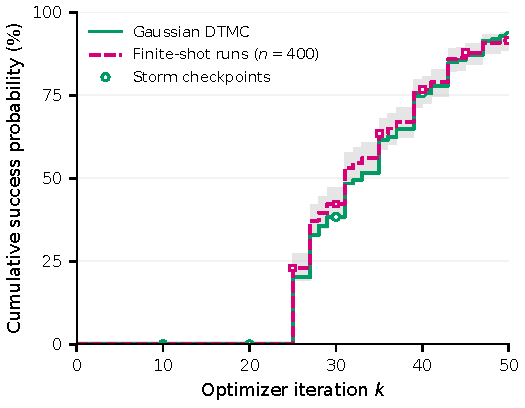
\includegraphics[width=\columnwidth]{figures/probability-comparison.pdf}
\caption{Cumulative probability of first satisfying $E_{\rm ideal}(z)-E_{\rm ref}\leq\GapThreshold$ versus optimizer update. The solid staircase is Gaussian-DTMC forward propagation, circles are Storm checkpoints, and the dashed staircase is the matched ideal-Born finite-shot experiment with \BaselineRuns independent seeded runs and \ShotsPerGroup shots per group/candidate. The shaded region gives marginal 95\% Wilson intervals at each update; it is not a simultaneous confidence band. No backend noise is included.}
\label{fig:probability-comparison}
\end{figure}

At the primary bound, \SuccessRuns/\BaselineRuns runs succeed and \BudgetRuns terminate normally at budget. The empirical probability is \PrimaryEmpiricalPercent\%, with Wilson interval [\PrimaryCILower\%, \PrimaryCIUpper\%], compared with \PrimaryModelPercent\% modeled probability. The absolute difference is \PrimaryDeviationPP percentage points. Table~\ref{tab:probabilities} gives exact checkpoint counts, intervals, deviations, and the supporting multiplicity-adjusted comparisons. Agreement denotes statistical compatibility at the tested resolution, not equality of distributions.

\begin{table*}[!t]
\centering\footnotesize
\caption{Final matched P1 results. Probabilities and Wilson limits are percentages; deviations are percentage points. Holm values adjust the informative checkpoint and P2 comparisons jointly. The early zero-probability checkpoints are structural, not independent empirical confirmation.}
\label{tab:probabilities}
\begin{tabular}{@{}rrrrlrr@{}}\toprule
$k$ & Successes/runs & Model (\%) & Empirical (\%) & Wilson 95\% (\%) & $|\Delta p|$ (pp) & Holm $p$ \\
\midrule
10 & 0/400 & 0.00 & 0.00 & [0.00, 0.95] & 0.00 & -- \\
20 & 0/400 & 0.00 & 0.00 & [0.00, 0.95] & 0.00 & -- \\
30 & 169/400 & 38.39 & 42.25 & [37.51, 47.14] & 3.86 & 0.338 \\
40 & 307/400 & 75.63 & 76.75 & [72.37, 80.62] & 1.12 & 0.627 \\
50 & 366/400 & 92.80 & 91.50 & [88.36, 93.85] & 1.30 & 0.627 \\
\bottomrule


\end{tabular}
\end{table*}

P2 is \PModelMean modeled updates conditional on success versus \PEmpiricalMean empirical updates, with the original percentile-bootstrap interval [\PMeanLow, \PMeanHigh]. Table~\ref{tab:conditional} preserves that interval, which does not contain the model mean. The earlier automated report therefore labeled P2 and P3 disagreements using marginal interval containment. The audit identified this as a statistical false alarm: the recomputed raw P2 $p$-value is \PMeanRawP, becoming \PMeanAdjustedP after adjustment. No informative comparison rejects at the family level. The corrected classifications are agreement through statistical compatibility for P2 and the derived P3; the original archived verdict remains unchanged for provenance. A non-rejection supplies neither an equivalence proof nor evidence that the model lies inside every marginal interval.

\begin{table*}[!t]
\centering\footnotesize
\caption{Conditional successful-path resources in the final matched experiment, based on \SuccessRuns successful executions. Intervals are the original 95\% percentile-bootstrap intervals from \BootstrapSamples resamples. P2 is statistically compatible after Holm adjustment; P3 scales P2 by \ShotsPerUpdate shots/update and is not an independent test.}
\label{tab:conditional}
\begin{tabular}{@{}lrrlrl@{}}\toprule
Contract / unit & Model mean & Empirical mean & Bootstrap 95\% & Absolute deviation & Holm $p$ \\
\midrule
P2: iterations & 33.111 & 32.290 & [31.579, 32.995] & 0.822 & 0.094 \\
P3: shots & 305,152.7 & 297,581.1 & [291,034.2, 304,077.6] & 7,571.6 & derived \\
\bottomrule


\end{tabular}
\end{table*}

Including unsuccessful runs, mean expenditure is \UnconditionalEmpirical updates versus \UnconditionalModel modeled updates. Total shot consumption above includes budget-terminated paths; it must not be confused with the cost conditioned on success. The primary probability comparison's approximate normal-theory deviation detectable at 80\% power is \DetectablePP percentage points at the sample size used here. This is a local planning approximation, not an equivalence margin or a statement that smaller deviations have been excluded. Supporting checkpoints are correlated, and the confidence band is pointwise.

The earlier FakeJakarta density-matrix study has \NoisySuccess/\NoisyRuns successes (\NoisyPercent\%). Its backend noise and compiled circuits fall outside the ideal Gaussian assumptions. We retain it as an out-of-model robustness observation, separate from the matched curve; its gap from the Gaussian prediction is not an estimate of Gaussian approximation error. Independent large-sample audit simulations support the auditor's false-alarm conclusion, but their saved arrays are absent from this workspace. We therefore do not plot them or reproduce their numerical summaries as newly verified paper results.

\subsection{Faults and Cross-Stage Discrepancies}
\label{sec:faults}
Table~\ref{tab:faults} reports all deterministic runtime verdicts, rather than only the expected target contract. There are \FaultClasses fault scenarios, each repeated \FaultRepetitions times, for \FaultRuns tests. Execution faults use the first update/candidate boundary; they do not represent diverse injection sites. The missing-evidence scenario deletes counts from a saved trace and retains the corresponding control execution. Thus it assesses evidence handling rather than an execution fault.

\begin{table*}[!t]
\centering\footnotesize
\caption{Full final fault verdict vectors. A: AGREEMENT; D: DISAGREEMENT; M: ASSUMPTION\_MISMATCH; I: INCONCLUSIVE. ``Target'' counts the expected target-contract verdict; ``DV pass'' is the independent temporal replay count. Each row is one scenario repeated with different count streams. Missing evidence is a saved-trace mutation. Its L1 D is an audited evidence-classification artifact, not proof of a physical ordering violation.}
\label{tab:faults}
\begin{tabular}{@{}lrrrrrrrrrr@{}}\toprule
Fault & Target & L1 & L2 & L3 & L4 & N1 & N2 & N3 & N4 & DV pass \\
\midrule
coefficient swap & 10/10 & A & A & A & A & A & D & A & A & 10/10 \\
corrupt energy & 10/10 & A & A & A & A & A & D & A & A & 10/10 \\
missing counts & 10/10 & D & I & A & A & I & I & I & I & 10/10 \\
premature commitment & 10/10 & I & D & A & A & I & I & A & A & 0/10 \\
shot mismatch & 10/10 & A & A & A & A & A & I & M & A & 10/10 \\
\bottomrule


\end{tabular}
\end{table*}

Premature commitment is caught by Python and DejaVu ordering checks. Altering the energy or coefficient pairing violates N2 while temporal projections pass, illustrating the different scopes. A shot-allocation change produces an N3 assumption mismatch and makes the probabilistic comparison inapplicable. Its fault-record applicability label is configured by the injector; it should not be advertised as an independently inferred stochastic verdict.

Missing counts make numeric reconstruction inconclusive. The current checker also records an L1 disagreement because its completeness condition conflates unavailable evidence with observed missing measurements. We retain the full vector and qualify this behavior: a deleted record alone does not establish that the original execution aggregated too early. The final data therefore support all expected target detections, but do not support flawless discrepancy classification or broad fault coverage. Terminal-boundary, stale-input, and additional injection-location coverage remain outside this suite.

\subsection{Answers to the Research Questions}
The contract matrix and frozen record answer RQ1 through explicit, inspectable mappings. For RQ2, logical model checking, mathematical numeric proofs, Gaussian reachability, runtime conformance, and empirical estimates each establish a different result with stated assumptions. For RQ3, the matched baseline supports logical/numeric agreement for the prospectively checked subclaims and probabilistic compatibility after the corrected statistical interpretation. L4's prospective gap prevents a stronger termination-reason claim. For RQ4, the fault vectors and separate cost measurements quantify the tested coverage and expense, without comparing tools on incompatible workloads or claiming complete fault detection.

\section{Related Work}
VQE and variational hybrid algorithms motivate the repeated interaction between classical decisions and quantum measurements~\cite{peruzzo2014,mcclean2016}. Their energy-estimation objective supplies the numeric obligation, while uncertainty and bounded search motivate the probabilistic one. NuXmv, Dafny, Storm, and DejaVu provide established model-checking, deductive-verification, probabilistic-analysis, and temporal-monitoring mechanisms~\cite{nuxmv,dafny,storm,dejavu}. Our contribution concerns their contract traceability and two-stage use in an implemented hybrid workflow; it is not a new proof engine or a formalism identifying their guarantees.

Statistical intervals and multiple-comparison control address a different inference problem from formal verification. Wilson intervals describe a binomial proportion~\cite{wilson}; Holm adjustment controls the family-wise rejection rate for a specified family of tests~\cite{holm}. Neither converts observed conformance into exhaustive correctness. The P2 correction illustrates why contract agreement must distinguish a stochastic observation, a marginal test, and the interpretation of related comparisons.

\section{Discussion and Limitations}
\label{sec:limitations}
\emph{Verification scope.} NuXmv is exhaustive for its encoded controller; Dafny proves kernels under mathematical semantics and preconditions; Storm is exhaustive for the constructed Gaussian DTMC. Runtime checking covers observed instrumented traces. Repeated executions provide statistical evidence. There is no theorem proving refinement of all projections to the Python program or composing them into unconditional correctness.

\emph{Trusted base.} Circuit and measurement-basis generation, bit order and parity interpretation, event instrumentation, proof tools, and the runtime reference checker are trusted. Hashes bind the artifacts to the recorded experiment but do not authenticate that counts originated from a physical backend. Consistent fabrication or relabeling is outside the claimed protection. The normal-CDF approximation and quadrature have no certified global stochastic-error bound.

\emph{Generality and observability.} The canonical instance is a small two-qubit benchmark with a fixed finite grid, ideal statistics, and an exact-energy stopping oracle. Its ideal target, cyclic optimizer, grouped measurements, and finite budget limit transfer to hardware or other VQE instances. The separate hardware and larger numeric traces demonstrate particular checks, not a matched cross-stage guarantee for those executions.

\emph{Statistical and audit boundaries.} The P2/P3 correction is disclosed as post-audit. Original marginal intervals and observations remain visible. Sample size constrains resolution, and a non-rejection is not equivalence. Development runs reused seeds and are excluded from sample counts. The independent audit found useful specification gaps, including termination reasons and evidence classification; this draft narrows claims rather than implying those frozen sources were repaired. Missing audit arrays and unretained scalability exports are documented in the reproducibility manifest.

\emph{Closed-loop scope.} The framework detects inconsistencies and supports revising assumptions or contracts before another sealed execution. The implemented feedback is manual. Its gated workflow does not test all possible combinations of prospective failure and runtime behavior, and its fault scenarios cover a limited boundary.

\section{Conclusion}
The two-stage framework connects family-owned VQE contracts to prospective results and concrete runtime evidence through a frozen canonical configuration. The final matched experiment supports contract-wise consistency within the stated logical and numeric subclaims and statistical compatibility of bounded Gaussian predictions and finite-shot observations, including the corrected P2/P3 interpretation. Full fault vectors and separately configured cost studies identify both useful checks and evidence limits. The result is an auditable relationship among heterogeneous verification layers, with obligations, assumptions, and interpretations kept explicit.

\balance
\section*{Artifact Availability}
The local reproducibility bundle includes this source, vector figures, editable architecture source, figure-generation scripts, generated numerical tables, \path{FIGURE_PLAN.md}, \path{FIGURE_MANIFEST.md}, and \path{PAPER_RESULT_TRACEABILITY.md}. The source manifest records hashes of the final assurance record, models, proof logs, raw traces, and retained layer-specific inputs. Original experimental artifacts are preserved; no public archive or DOI is claimed.

\bibliographystyle{IEEEtran}
\bibliography{references}
\end{document}
